\documentclass[11pt,a4paper]{article}
\usepackage[margin=1in]{geometry}
\usepackage[T1]{fontenc}
\usepackage[utf8]{inputenc}
\usepackage{lmodern}
\usepackage{graphicx}
\usepackage{booktabs}
\usepackage{array}
\usepackage{longtable}
\usepackage{tabularx}
\usepackage{xcolor}
\usepackage{hyperref}
\usepackage{enumitem}
\usepackage{float}
\usepackage{amsmath}
\hypersetup{colorlinks=true, linkcolor=blue, urlcolor=blue, citecolor=blue}

\title{UQ-QNN Repository Overview, Development Progress, and Rerun Experiment Analysis}
\author{Project Presentation Notes}
\date{April 2, 2026}

\begin{document}
\maketitle
\tableofcontents
\newpage

\section{Repository Content and Goal}

The repository \texttt{uq-qnn} implements a framework for \emph{uncertainty-aware photonic quantum neural networks}. The core goal is to train photonic circuits such as Clements meshes and memristive photonic variants on regression and classification tasks while preserving a practical workflow for:

\begin{itemize}[leftmargin=*]
    \item differentiable training via the parameter-shift rule (PSR),
    \item reproducible experiment execution and reporting,
    \item support for both fast analytical simulation and full Perceval-based simulation,
    \item uncertainty quantification through repeated noisy forward passes,
    \item controlled comparisons between standard photonic circuits and memristive circuits.
\end{itemize}

At a high level, the data flow is:
\[
    x \rightarrow \phi(x)=2\arccos(x) \rightarrow \text{photonic circuit} \rightarrow \text{Born-rule probabilities} \rightarrow \text{loss} \rightarrow \text{PSR gradients}.
\]

The repository now contains three complementary layers:
\begin{enumerate}[leftmargin=*]
    \item \textbf{Modeling and simulation}: Clements circuits, memristive feedback, singles/coincidence measurements, NumPy and Perceval backends.
    \item \textbf{Training and experimentation}: \texttt{SimConfig}, \texttt{Experiment}, uncertainty analysis, metrics, artifact export.
    \item \textbf{Analysis and communication}: reproducible report folders, comparison scripts, benchmark scripts, and now this presentation material.
\end{enumerate}

\section{Project Stages and Progress}

The changelog shows a clear staged evolution from a collection of scripts toward a structured research codebase.

\subsection{Stage 1: Baseline simulation and PSR training}
The original codebase established the photonic training loop: circuit simulation, Born-rule outputs, and PSR-driven optimization. This stage proved that Clements-style photonic networks could be trained on synthetic tasks, but the workflow was still script-heavy and difficult to compare across runs.

\subsection{Stage 2: Experiment API and reproducibility}
A major step was the introduction of the \texttt{Experiment} API and explicit script-local configuration. This changed the repository from a collection of ad hoc scripts into a reproducible framework with:
\begin{itemize}[leftmargin=*]
    \item timestamped run folders,
    \item saved metrics and artifacts,
    \item centralized logging,
    \item a consistent mapping from configuration to training and inference.
\end{itemize}
This stage directly advanced the goal of making uncertainty-aware photonic experiments repeatable and comparable.

\subsection{Stage 3: Hardware abstraction and cleaned interfaces}
The next stage introduced hardware profiles and a cleaner separation of concerns. With this, the repository could represent ideal and noisy hardware conditions without rewriting experiment scripts. In parallel, dead legacy utilities and configuration indirection were removed. This moved the project closer to realistic photonic deployment scenarios.

\subsection{Stage 4: PhotonicCircuit facade and package cleanup}
The addition of \texttt{PhotonicCircuit}, public circuit helpers, and a simulation package reorganization improved code clarity and reduced duplicated logic. This stage made the fast analytical backend easier to use directly and made the architecture more maintainable.

\subsection{Stage 5: Correctness and developer quality}
Further work tightened typing, fixed edge cases in hardware noise and memristive uncertainty handling, and added regression tests. This stage matters because the research questions in the repository are sensitive to subtle simulator and gradient issues.

\subsection{Stage 6: Fast memristive NumPy backend and targeted reruns}
The latest work targeted a key bottleneck: memristive NumPy simulations were correct but slow because they rebuilt full unitaries at every step. We introduced an optimized state-propagation path for memristive singles runs, first for discrete mode and then for swipe mode. To evaluate both the engineering change and the modeling consequences, we reran and added several experiments focused on memristive circuits.

\section{What We Changed to Reach the Goals}

The repository goals were not reached through one single feature but through a sequence of structural and experimental changes.

\subsection{Workflow changes}
\begin{itemize}[leftmargin=*]
    \item Replaced hidden global configuration with explicit per-script \texttt{CONFIG} dictionaries.
    \item Added the \texttt{Experiment} context manager to standardize training, prediction, uncertainty, logging, and artifact saving.
    \item Moved results into timestamped report folders with \texttt{run\_summary.json} to support later analysis and presentation.
\end{itemize}

\subsection{Architecture and simulator changes}
\begin{itemize}[leftmargin=*]
    \item Promoted public circuit helpers such as memristive index normalization and phase-to-MZI mapping.
    \item Added \texttt{PhotonicCircuit} as a lightweight interface for fast NumPy simulations.
    \item Refactored simulation code into a clearer package with a dedicated memristive state manager.
\end{itemize}

\subsection{Correctness and robustness changes}
\begin{itemize}[leftmargin=*]
    \item Fixed classification and scalar-noise edge cases.
    \item Corrected gradient handling for memristive weights.
    \item Added more tests to protect against behavioral regressions.
\end{itemize}

\subsection{Performance changes}
The most recent change is especially important for the current research direction:
\begin{itemize}[leftmargin=*]
    \item a dedicated fast NumPy memristive singles path now propagates a single-photon state vector through the Clements mesh instead of rebuilding a full unitary at each step,
    \item this path supports both discrete and swipe-mode memristive runs,
    \item targeted regression tests verify parity with the previous slower loop.
\end{itemize}

This performance work was necessary because investigating memristor placement and multi-memristor configurations becomes much more expensive if every rerun must pay the old simulation cost.

\section{Rerun Experiments Considered in This Document}

This document focuses on the reruns and new experiments created during the latest memristor investigation:
\begin{enumerate}[leftmargin=*]
    \item \textbf{Function and memristor comparison}: standard vs. memristive architecture across several synthetic functions.
    \item \textbf{Smooth-step placement comparison}: one memristor placed at several different phase positions.
    \item \textbf{Smooth-step multi-memristor comparison}: no memristor, one memristor, or two memristors.
    \item \textbf{Memristive backend benchmark}: fast NumPy memristive path vs. the legacy reference loop.
\end{enumerate}

The corresponding report folders are:
\begin{itemize}[leftmargin=*]
    \item \texttt{reports/function\_and\_memristor\_comparison/2026-04-01\_212859/}
    \item \texttt{reports/smooth\_step\_memristor\_placement\_comparison/2026-04-01\_223609/}
    \item \texttt{reports/smooth\_step\_multi\_memristor\_comparison/2026-04-01\_230245/}
    \item \texttt{reports/memristive\_backend\_benchmark/2026-04-01\_215523/}
\end{itemize}

\section{Experiment 1: Function and Memristor Comparison}

This rerun compares a standard 6-mode Clements mesh to a 6-mode memristive variant with one memristive phase. The goal was to answer a basic modeling question: \emph{does the memristor help function fitting across representative regression targets?}

\subsection{Selected results}

\begin{table}[H]
\centering
\begin{tabular}{lrrrr}
\toprule
Function & Standard RMSE & Memristor RMSE & Standard $R^2$ & Memristor $R^2$ \\
\midrule
Quartic & 0.0200 & 0.0342 & 0.9876 & 0.9637 \\
Sinusoid & 0.0274 & 0.0210 & 0.9455 & 0.9680 \\
Multi-modal & 0.1261 & 0.1236 & 0.2757 & 0.3043 \\
Smooth step & 0.0714 & 0.0754 & 0.8393 & 0.8209 \\
\bottomrule
\end{tabular}
\caption{Main fit metrics from the rerun function-vs-memristor comparison.}
\end{table}

\subsection{Analysis}
The memristor does \emph{not} provide a uniform advantage.
\begin{itemize}[leftmargin=*]
    \item It helps on the sinusoid and slightly improves the multi-modal case in terms of RMSE/$R^2$.
    \item It hurts on quartic and smooth step.
    \item Calibration behavior remains unstable; for example the smooth-step memristor run shows substantially worse NLL and very poor 95\% coverage.
\end{itemize}

This experiment led to the next question: perhaps the issue is not memristive feedback itself, but \emph{where} the memristor is placed in the 6-mode mesh.

\begin{figure}[H]
    \centering
    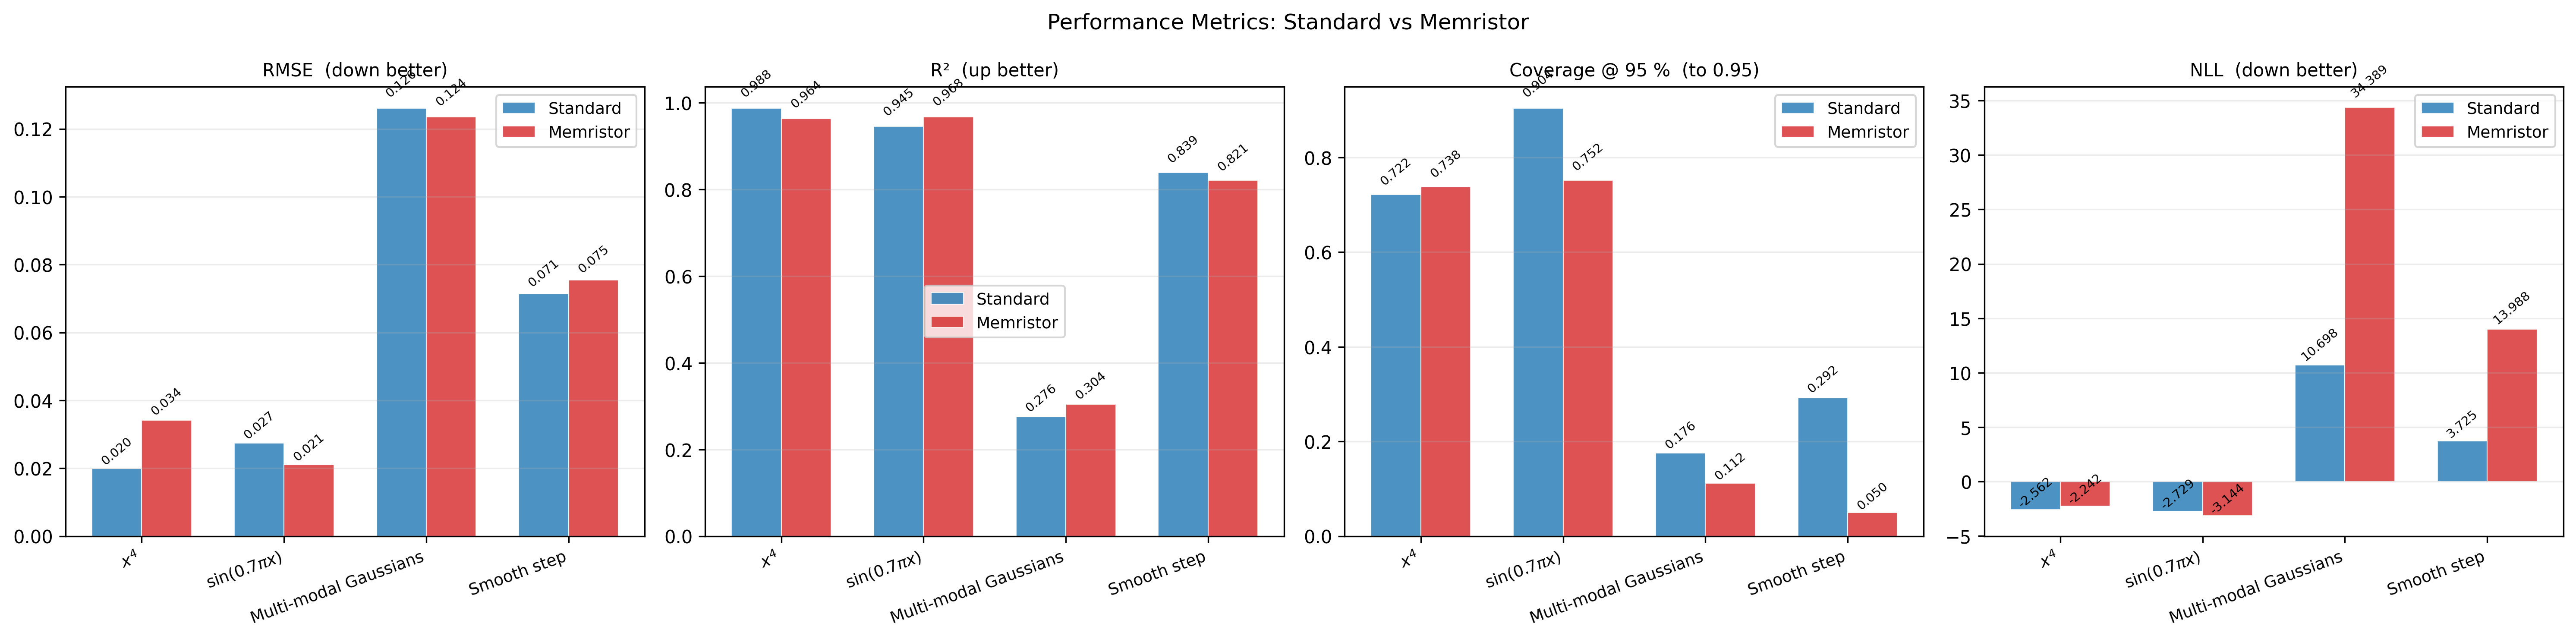
\includegraphics[width=0.9\textwidth]{../reports/function_and_memristor_comparison/2026-04-01_212859/metrics_comparison.png}
    \caption{Metrics from the function-and-memristor rerun.}
\end{figure}

\section{Experiment 2: Smooth-Step Memristor Placement Comparison}

The smooth-step function is a useful focused test because the earlier broad comparison suggested that a single memristor was not clearly helping on this task. We therefore reran the smooth-step problem while moving the memristor to different positions.

\subsection{Placements tested}
The following configurations were tested:
\begin{itemize}[leftmargin=*]
    \item no memristor (standard baseline),
    \item phase 0 on MZI(0,1),
    \item phase 2 on MZI(2,3),
    \item phase 4 on MZI(4,5),
    \item phase 6 on MZI(1,2),
    \item phase 8 on MZI(3,4).
\end{itemize}

\subsection{Key metrics}

\begin{table}[H]
\centering
\begin{tabular}{lrrrr}
\toprule
Placement & RMSE & $R^2$ & Coverage & NLL \\
\midrule
Standard & 0.0718 & 0.8377 & 0.368 & 3.790 \\
Phase 0 & 0.4038 & -4.1344 & 0.002 & 90936.430 \\
Phase 2 & 0.0712 & 0.8403 & 0.278 & 3.766 \\
Phase 4 & 0.0712 & 0.8403 & 0.278 & 3.766 \\
Phase 6 & 0.0757 & 0.8193 & 0.048 & 14.559 \\
Phase 8 & 0.0712 & 0.8403 & 0.278 & 3.766 \\
\bottomrule
\end{tabular}
\caption{Smooth-step placement rerun metrics.}
\end{table}

\subsection{Analysis}
This rerun gives a nuanced answer.
\begin{itemize}[leftmargin=*]
    \item The memristor \textbf{placement matters strongly}. Phase 0 is catastrophic and destabilizes the fit.
    \item Phases 2, 4, and 8 produce almost the same fit quality and are only marginally better than the standard baseline in RMSE/$R^2$.
    \item Phase 6 is worse than the standard baseline and dramatically worse in uncertainty coverage and NLL.
\end{itemize}

The most important conclusion is that the repository's memristive mechanism is not ``plug-and-play.'' A memristor can degrade the model if it is placed too close to the data encoding or in a part of the mesh where the feedback creates an unfavorable recurrent bias.

\begin{figure}[H]
    \centering
    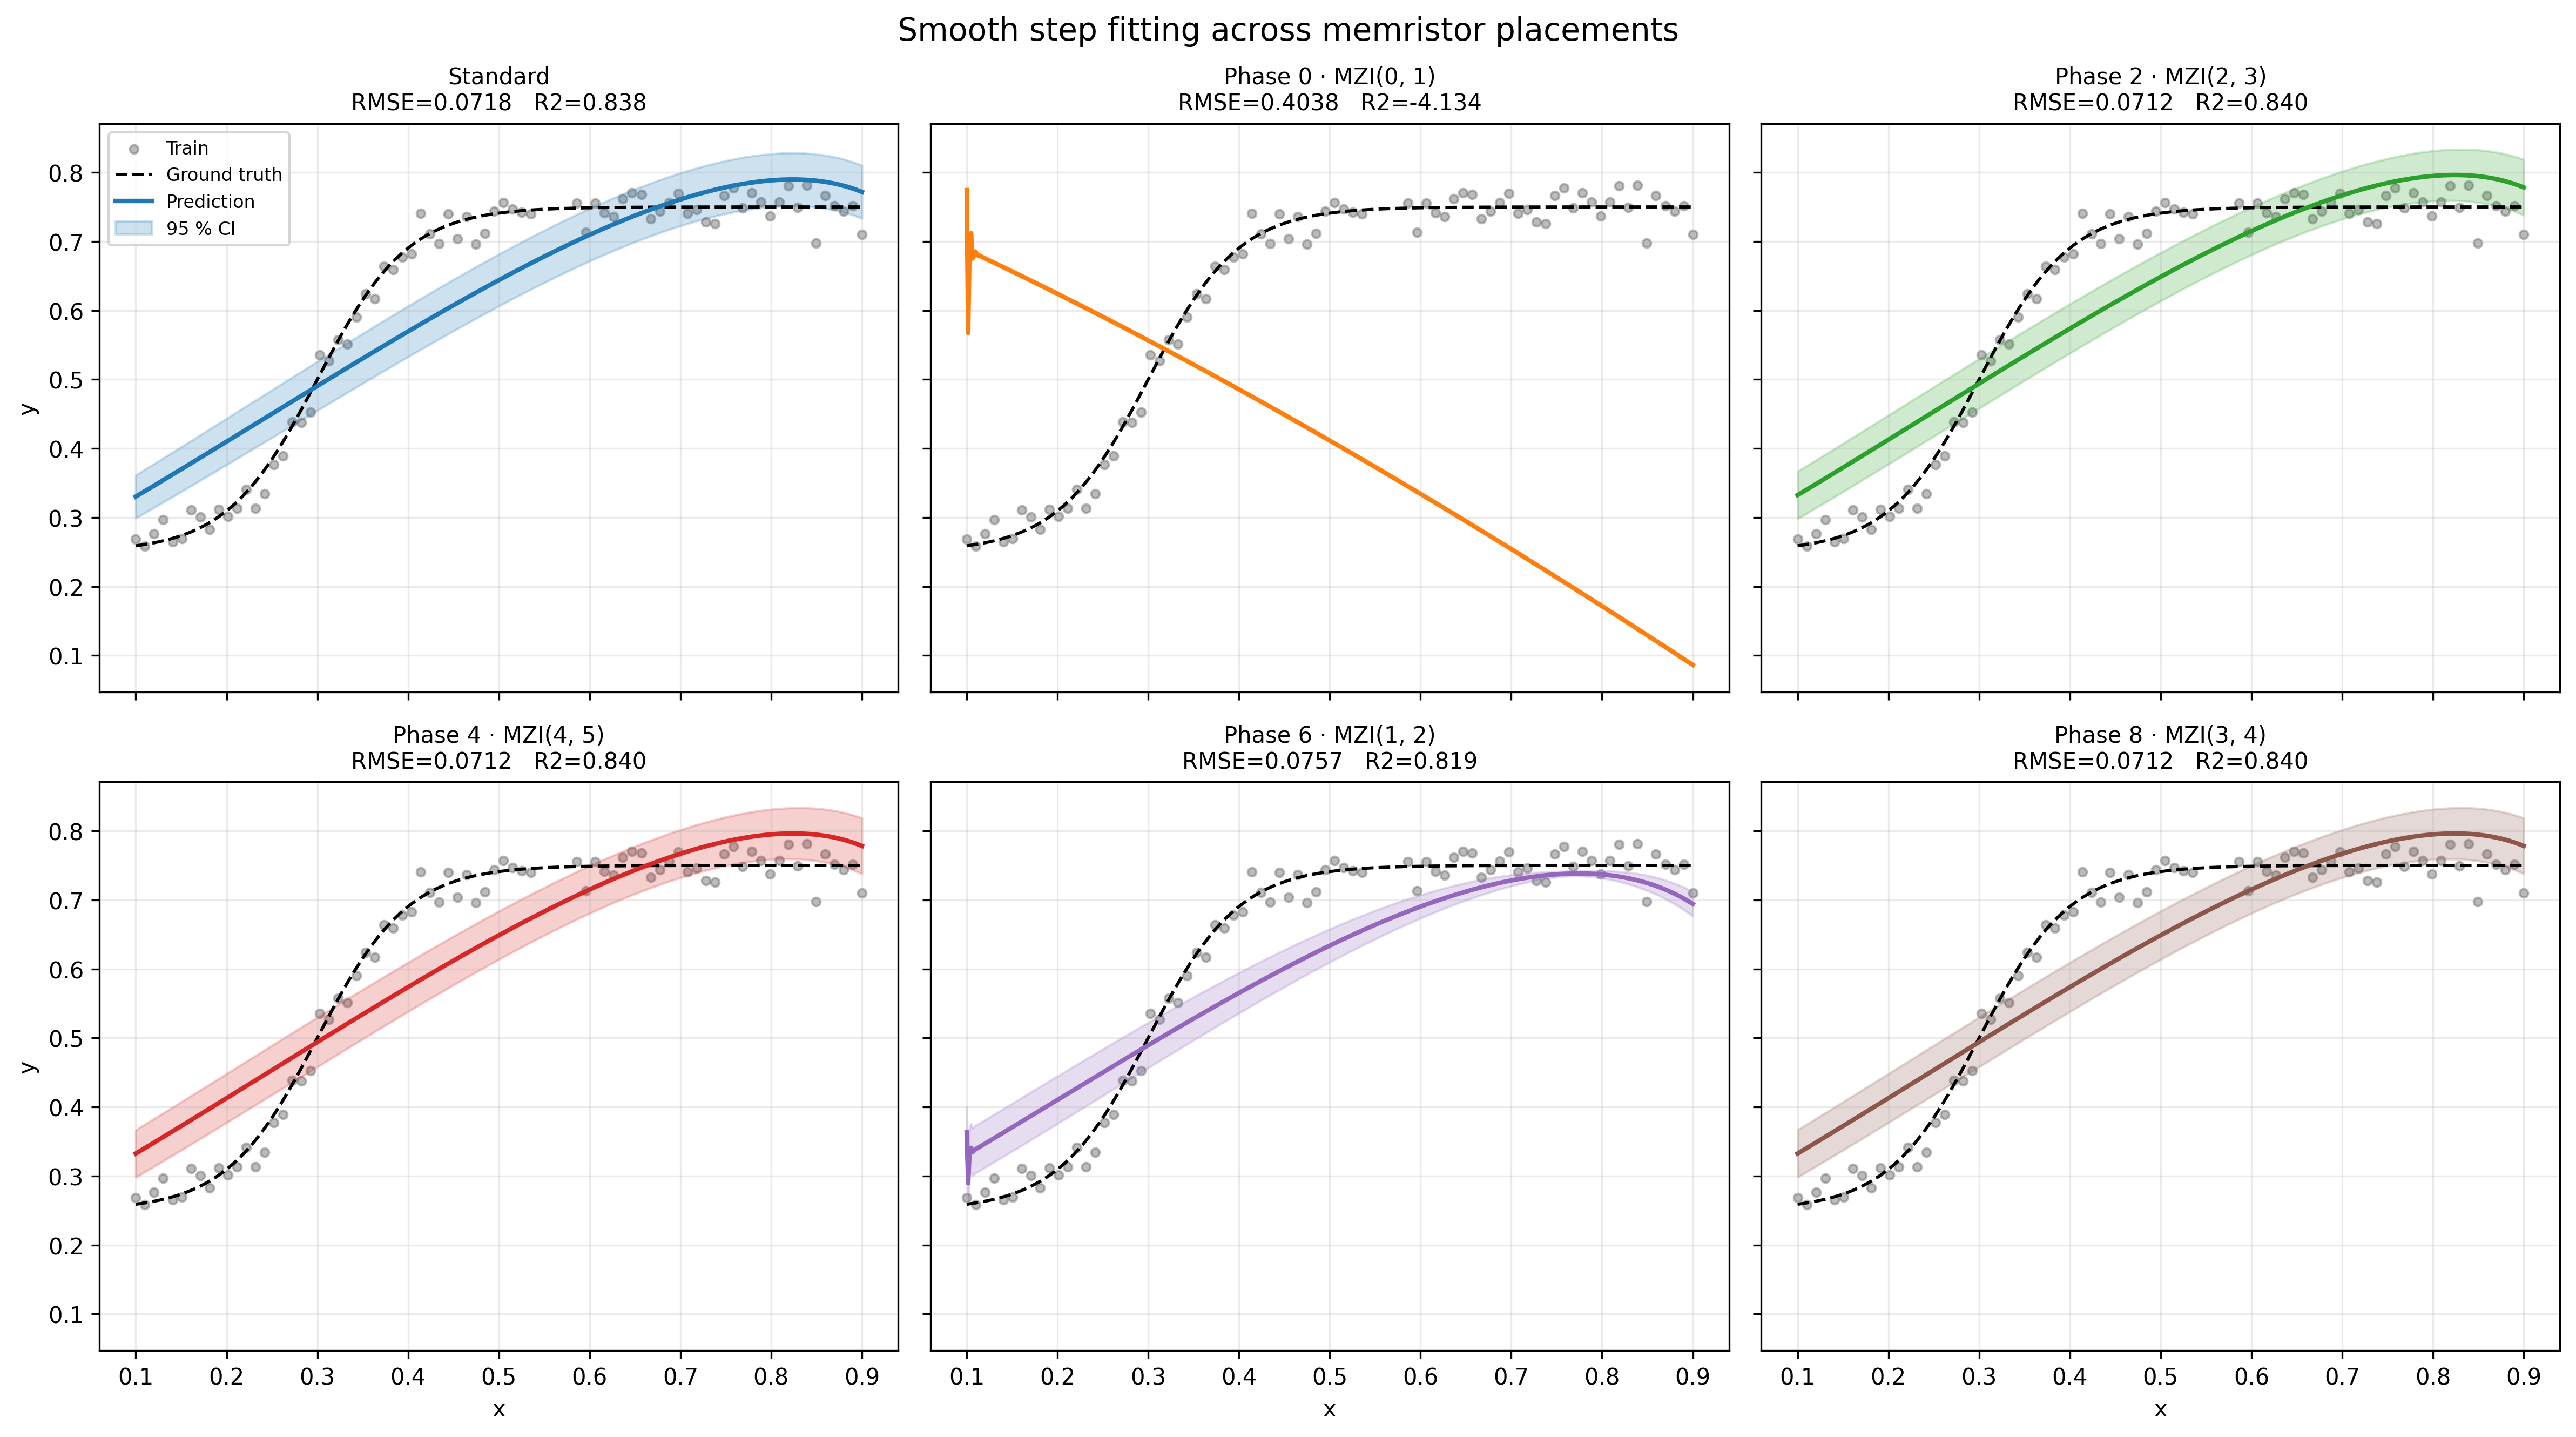
\includegraphics[width=0.9\textwidth]{../reports/smooth_step_memristor_placement_comparison/2026-04-01_223609/predictions_grid.png}
    \caption{Smooth-step fits for different memristor placements.}
\end{figure}

\section{Experiment 3: Smooth-Step Single vs. Multiple Memristors}

After the single-placement rerun, we tested whether adding \emph{more than one} memristor could recover a useful effect. The chosen pair was phases 6 and 8, corresponding to the MZI(1,2) and MZI(3,4) positions.

\subsection{Configurations}
\begin{itemize}[leftmargin=*]
    \item standard baseline,
    \item single memristor at phase 6,
    \item single memristor at phase 8,
    \item two memristors at phases 6 and 8.
\end{itemize}

\subsection{Results}

\begin{table}[H]
\centering
\begin{tabular}{lrrrr}
\toprule
Configuration & RMSE & $R^2$ & Coverage & NLL \\
\midrule
Standard & 0.0718 & 0.8377 & 0.368 & 3.790 \\
Single 6 & 0.0757 & 0.8193 & 0.048 & 14.559 \\
Single 8 & 0.0712 & 0.8403 & 0.278 & 3.766 \\
Double 6+8 & 0.0764 & 0.8164 & 0.052 & 12.595 \\
\bottomrule
\end{tabular}
\caption{Smooth-step single-vs-multiple memristor rerun metrics.}
\end{table}

\subsection{Analysis}
The two-memristor configuration did \emph{not} improve the smooth-step task.
\begin{itemize}[leftmargin=*]
    \item The best RMSE in this group comes from the standard baseline or the single memristor at phase 8, depending on whether one prioritizes accuracy or calibration.
    \item Adding the second memristor at phase 6 degrades the model relative to single phase 8.
    \item This suggests that the phase-6 feedback pathway is harmful in this task and remains harmful even when paired with another memristor.
\end{itemize}

So, the correct takeaway is not simply ``more memristors are better.'' Instead, memristive feedback seems highly task- and placement-dependent.

\begin{figure}[H]
    \centering
    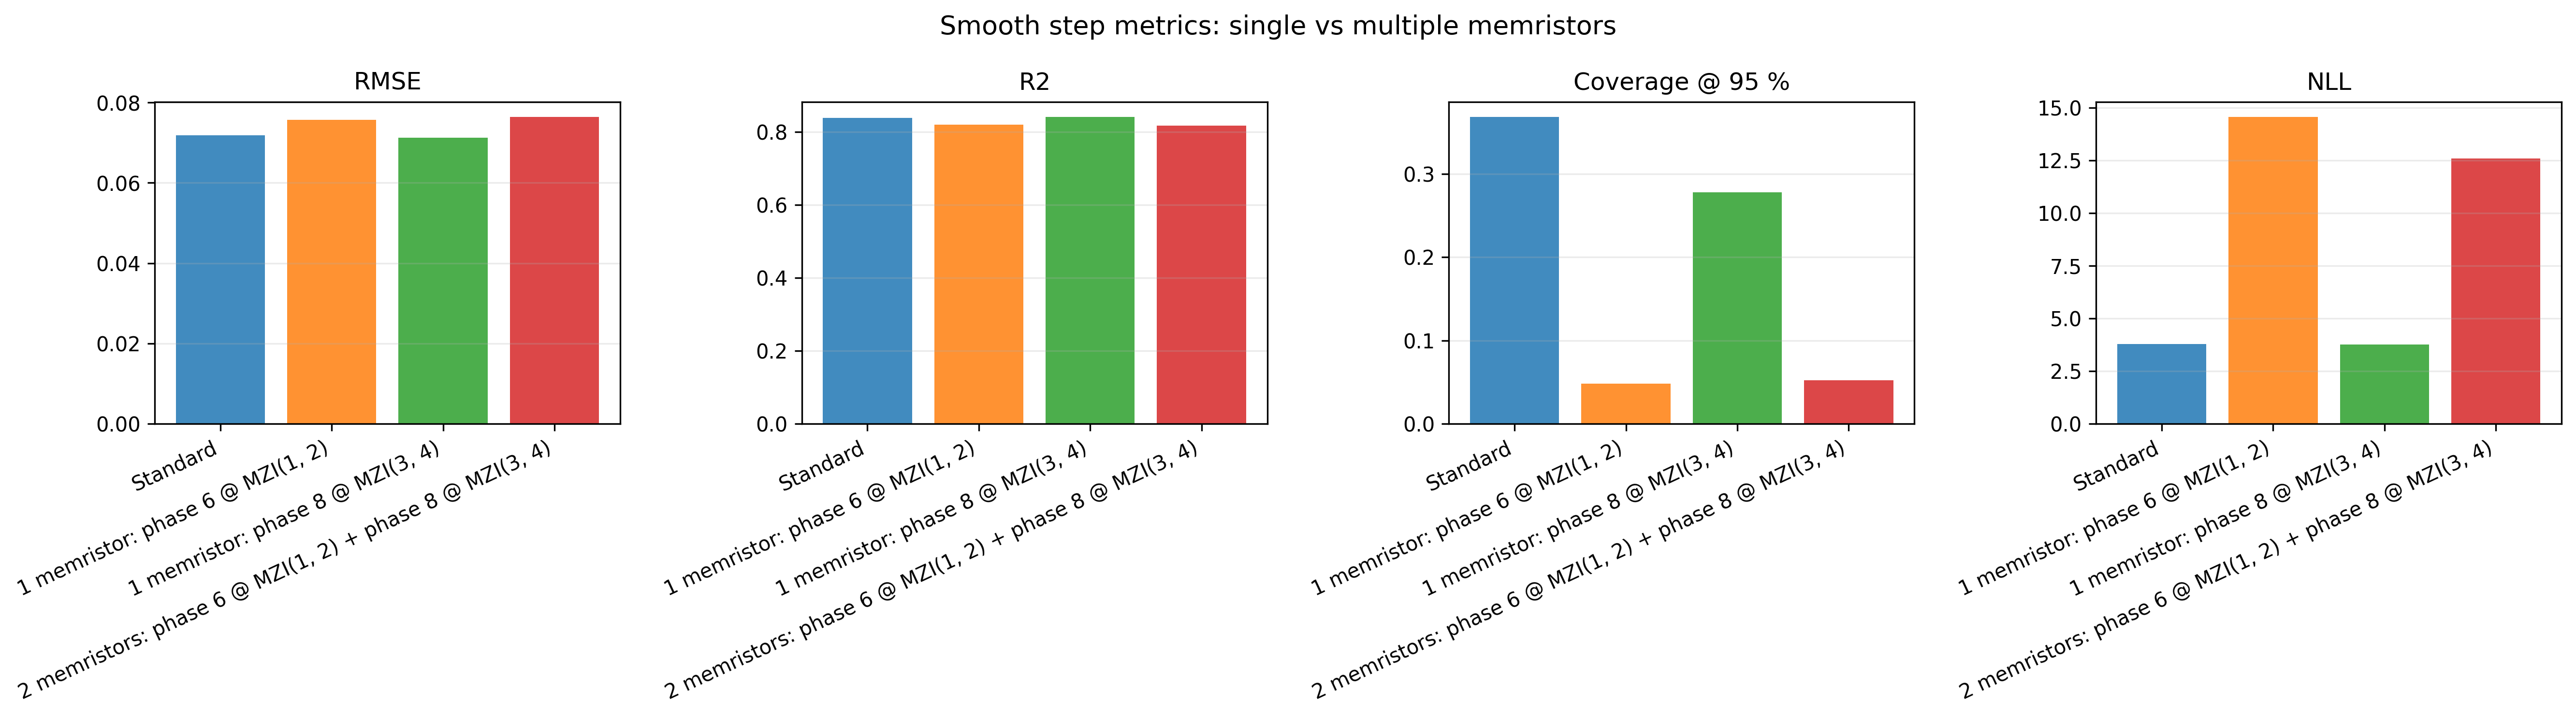
\includegraphics[width=0.9\textwidth]{../reports/smooth_step_multi_memristor_comparison/2026-04-01_230245/metrics_comparison.png}
    \caption{Smooth-step comparison for one vs. two memristors.}
\end{figure}

\section{Experiment 4: Memristive Backend Benchmark}

The repository work was not only about modeling; it also targeted simulator efficiency. We benchmarked the new fast NumPy memristive backend against the previous reference implementation.

\begin{table}[H]
\centering
\begin{tabular}{lrrrr}
\toprule
Case & Fast [ms] & Legacy [ms] & Speedup & Notes \\
\midrule
Discrete & 5.562 & 22.994 & 4.13x & one memristor, no swipe \\
Swipe & 23.315 & 109.183 & 4.68x & memristive swipe mode \\
Swipe inline & 22.744 & 100.722 & 4.43x & inline encoding + swipe \\
\bottomrule
\end{tabular}
\caption{Benchmark of the fast memristive NumPy backend.}
\end{table}

\subsection{Analysis}
The performance change is meaningful for research iteration.
\begin{itemize}[leftmargin=*]
    \item The new backend yields roughly a 4.1x--4.7x runtime reduction on the tested workloads.
    \item The gain is especially important for swipe mode, where repeated sub-evaluations per data point make the old implementation expensive.
    \item Because parity tests were added, this acceleration does not trade away correctness.
\end{itemize}

\begin{figure}[H]
    \centering
    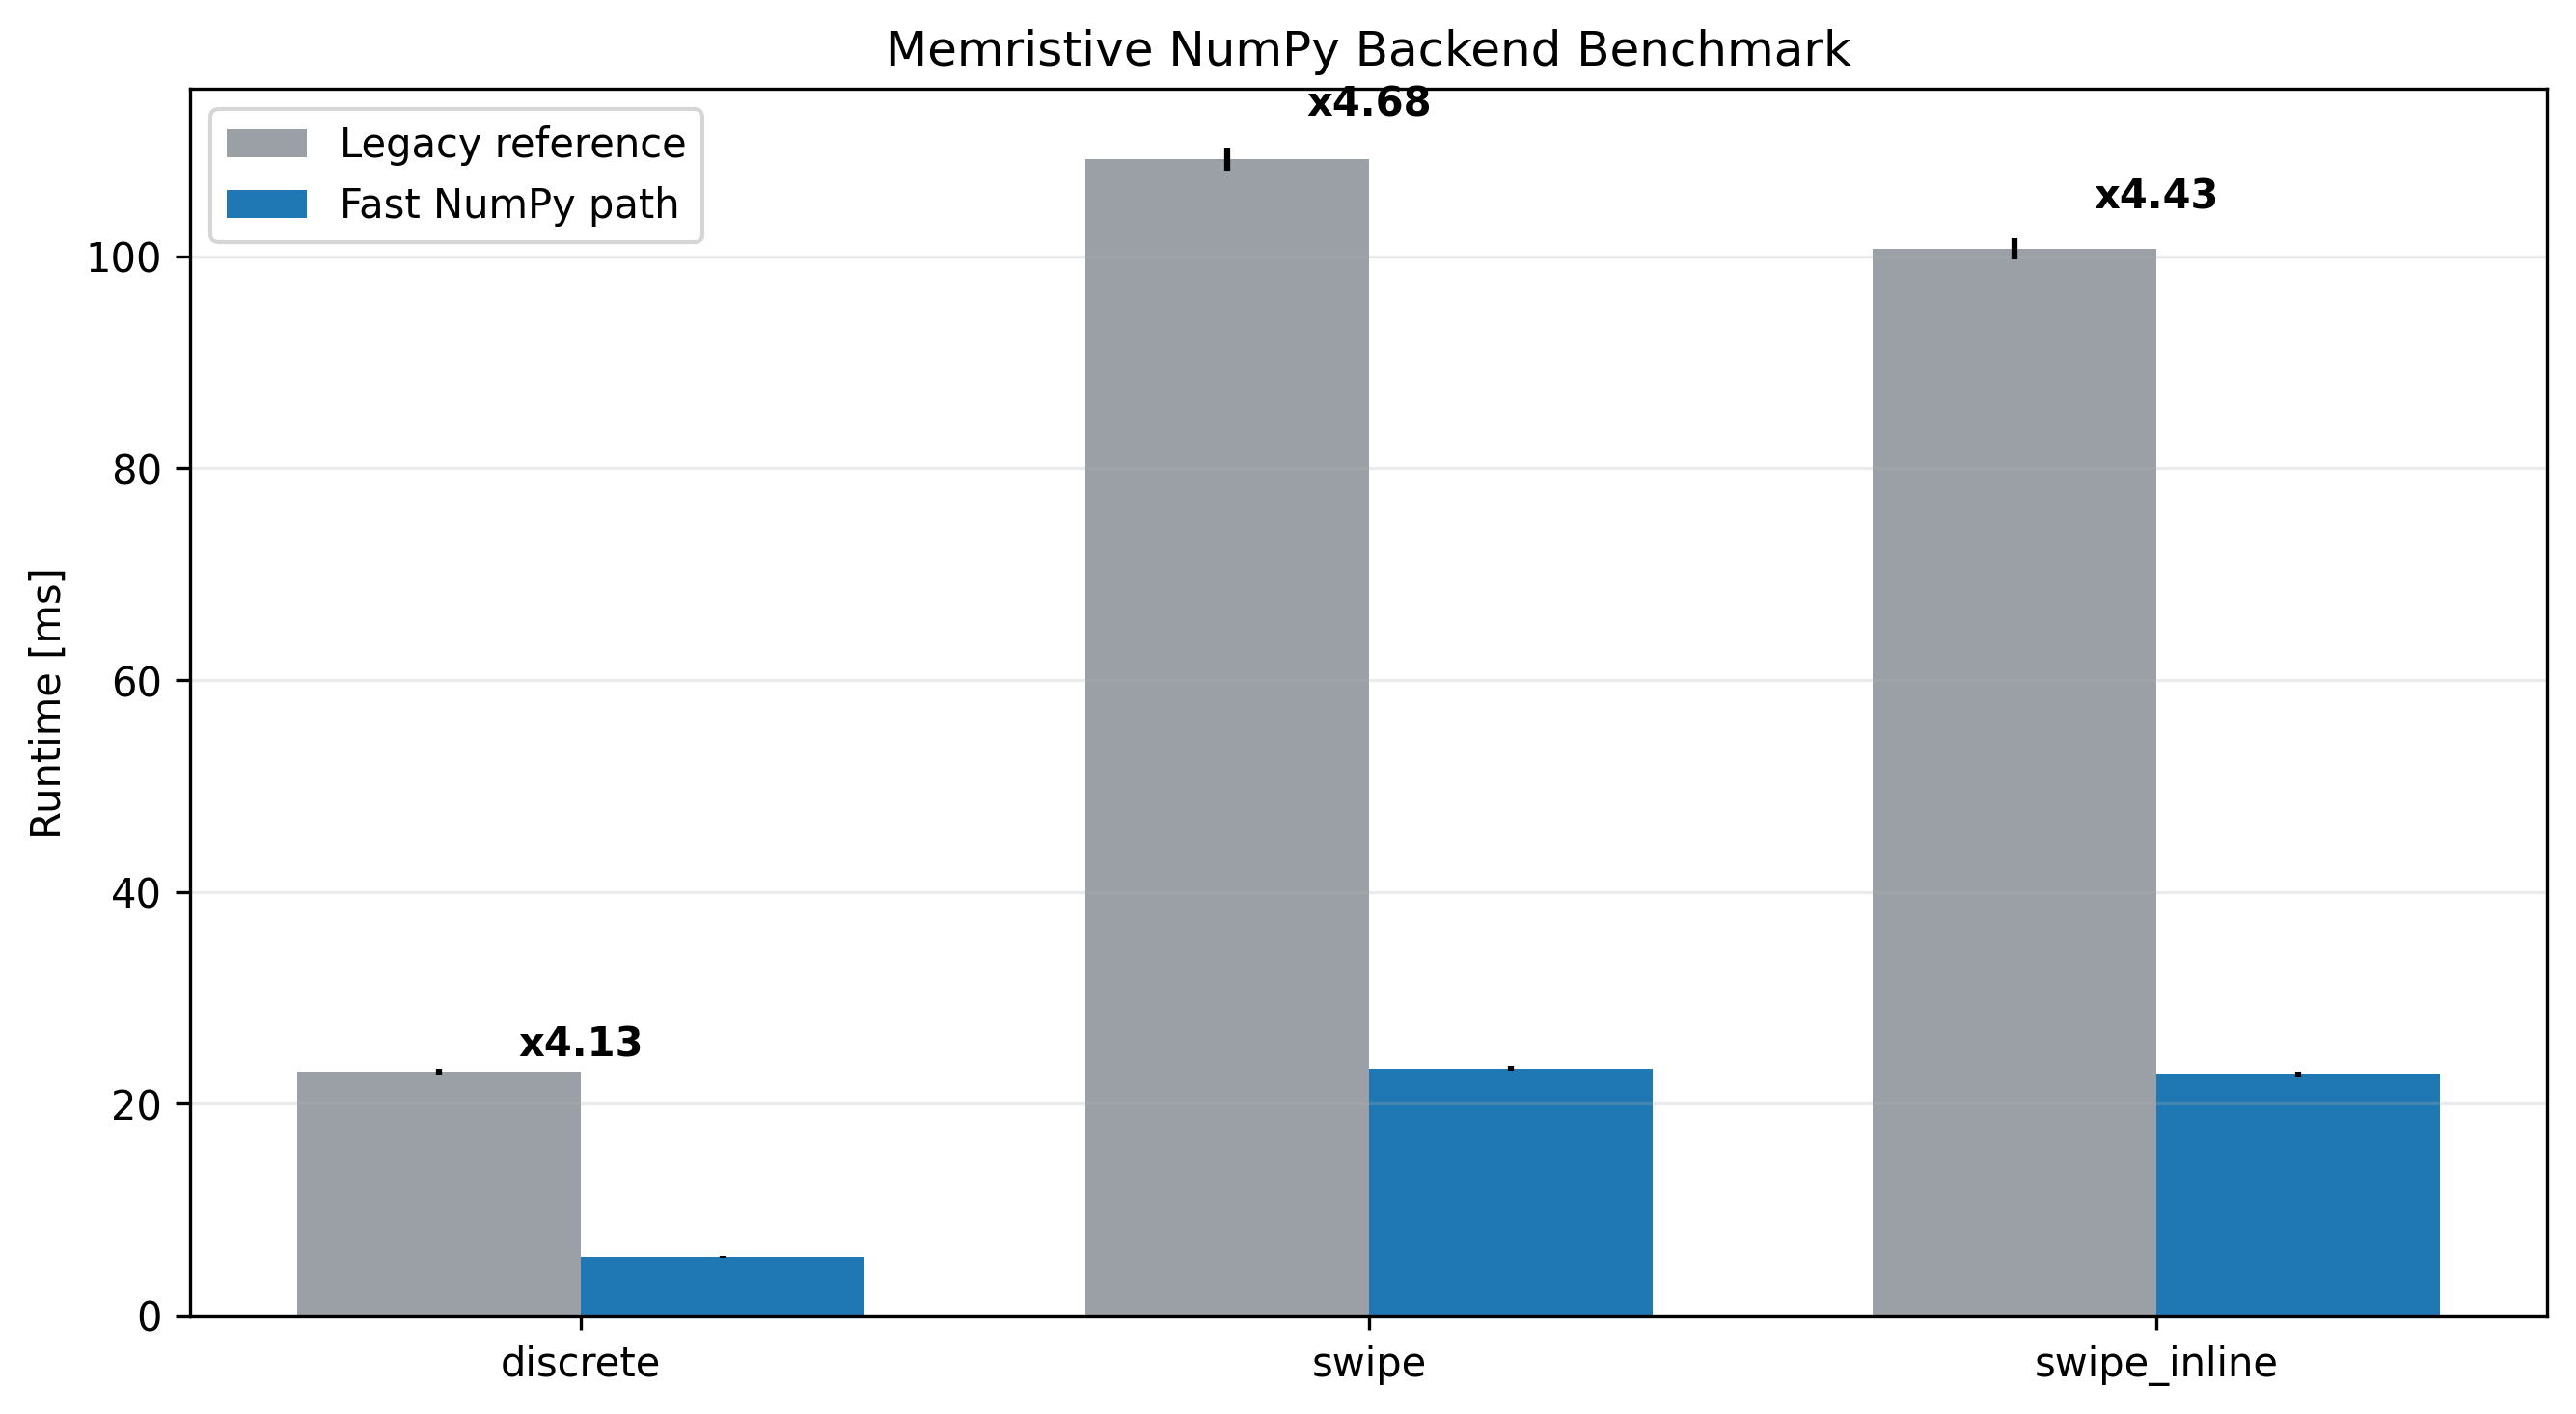
\includegraphics[width=0.75\textwidth]{../reports/memristive_backend_benchmark/2026-04-01_215523/memristive_backend_benchmark.png}
    \caption{Benchmark plot for the new memristive NumPy backend.}
\end{figure}

\section{Overall Conclusions from the Reruns}

The rerun experiments give a balanced picture of the current state of the repository.

\subsection{What worked}
\begin{itemize}[leftmargin=*]
    \item The repository now supports reproducible comparisons and benchmarking with minimal boilerplate.
    \item The new memristive NumPy backend significantly accelerates the practical workflow.
    \item Memristive feedback can improve some functions, especially periodic structure such as the sinusoid.
\end{itemize}

\subsection{What did not work as hoped}
\begin{itemize}[leftmargin=*]
    \item A single memristor is not universally beneficial.
    \item On smooth-step fitting, most memristor placements do not beat the standard baseline in a meaningful way.
    \item Two memristors at phases 6 and 8 do not improve the smooth-step task; in fact, they hurt relative to the best single-placement variant.
\end{itemize}

\subsection{Interpretation}
The engineering progress is clear: the framework is more modular, faster, better tested, and easier to analyze. The scientific result is more subtle: memristive photonic feedback does not automatically improve function fitting. Its value depends on task, placement, and uncertainty behavior. That is still a useful result, because it narrows the search space for future memristor studies.

\section{Recommended Next Steps}

Based on the reruns, the next stage should focus on \emph{structured exploration} rather than simply adding more memristors.

\begin{enumerate}[leftmargin=*]
    \item Test two-memristor pairs that avoid phase 6, since that position repeatedly produced poor results on smooth step.
    \item Extend the comparisons to harder targets where recurrence may be more naturally beneficial than on a simple smooth step.
    \item Study memory depth explicitly; placement and depth may interact.
    \item Add benchmark cases with multiple memristors so performance scaling is quantified alongside modeling quality.
    \item Continue using calibration metrics, not just RMSE/$R^2$, because some memristive runs appear accurate but poorly calibrated.
\end{enumerate}

\section{Build Notes}

This report can be compiled from the repository root with:
\begin{verbatim}
cd presentation
pdflatex repository_overview.tex
\end{verbatim}

The accompanying Beamer slide deck is stored as \texttt{rerun\_experiments\_slides.tex} in the same folder.

\end{document}
